\documentclass{article}
\usepackage{graphicx} %
\usepackage{tikz}
\usepackage{amsmath}
\usepackage{amssymb}
\usetikzlibrary{arrows}

\title{Gilbran Mahdavikia Raja}
\author{5025241134}

\begin{document}

\begin{flushleft}
    Gilbran Mahdavikia Raja \\
    5025241134 \\
\end{flushleft}
{\Large \textbf{5.4}}
\begin{description}
    \item[$47.$] Diberikan fungsi $f(x) = (x - 2)^{\frac{1}{3}}$. Dapatkan 
    \begin{description}
        \item[(d)] interval dimana kurva cekung ke bawah/ke atas
        \begin{itemize}
            \item[] $f(x) = (x - 2)^{\frac{1}{3}}$
            \item[$\Leftrightarrow$] $f'(x) = \frac{1}{3}(x - 2)^{-\frac{2}{3}}$
            \item[$\Leftrightarrow$] $f''(x) = -\frac{2}{9}(x - 2)^{-\frac{5}{3}}$
            \item[] $f''(x)$ tidak terdefinisi pada $x = 2$ karena $(x - 2)^{-\frac{5}{9}}$. Dengan demikian $x = 2$ adalah titik singular.
            \item[] 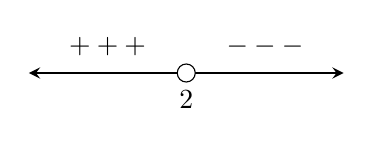
\begin{tikzpicture}[]
                \draw[thick, stealth-stealth] (-2,0) -- (2,0);
                \filldraw[fill=white] (-.0,0) circle (3.25pt) node[below,yshift=-.1cm] {$2$};
                \draw (1,0) node [above,yshift=.1cm] {$---$};
                \draw (-1,0) node [above,yshift=.1cm] {$+++$};
            \end{tikzpicture}
            \item[] jadi fungsi $f(x)$ cekung ke atas pada interval $(-\infty, 2)$ dan cekung ke bawah pada interval $(2, +\infty)$
        \end{itemize}
        \item[(e)] sketsa grafik $f(x)$
        \item[] \begin{description} 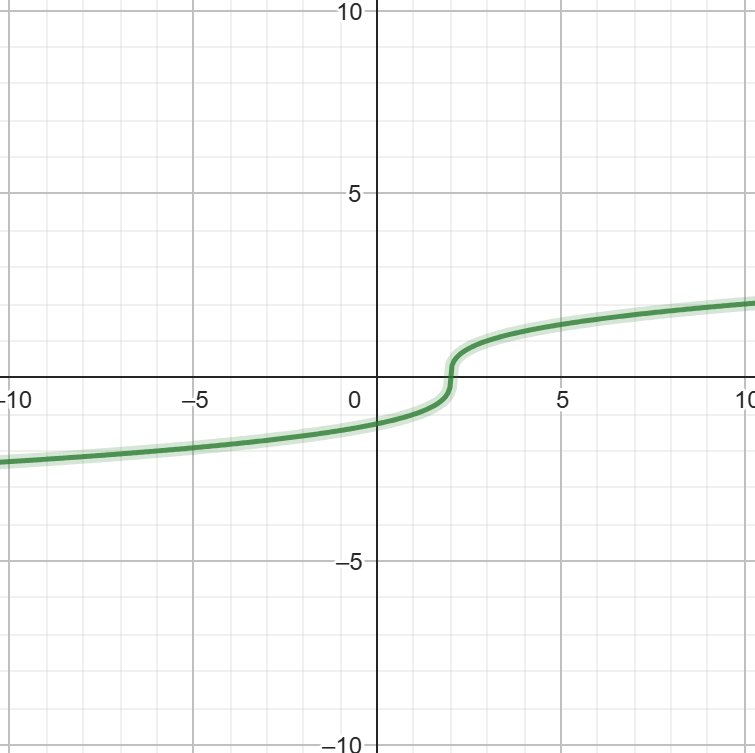
\includegraphics[scale=0.3]{img/1.png}\end{description}
    \end{description}
\end{description}

\end{document}